\documentclass[main.tex]{subfiles}
\ProvidesPackage{preamble}

\usepackage[nottoc]{tocbibind}
\usepackage[english]{babel}
\usepackage[utf8]{inputenc}
\usepackage[table]{xcolor}
\usepackage[nohead, nomarginpar, margin=1in, foot=.25in]{geometry}
\usepackage{tabularx}
\usepackage{graphicx}
\usepackage{float}
\usepackage[english]{babel}
\usepackage{paralist}
\usepackage{datetime}
\usepackage{afterpage}

\begin{document}

\section{Requirements}
Earlier in the inception phase of the development, we classified our requirements using the established FURPS+ model \cite{FURPS}. Since identifying requirements for our initial project report \cite{TR} we have also identified some additional requirements that Thalia should fulfil based on feedback from our project guide. Let us briefly revisit our main functional and non-functional requirements. The items outlined below focus on some of the key requirements we have so far identified as features necessary for providing a compelling product for paying customers.

\subsection{Functional Requirements}
 
{
\setlength{\tabcolsep}{30pt}
\renewcommand{\arraystretch}{2}
\centering
\rowcolors{2}{gray!25}{white}
\begin{tabularx}{\linewidth}{|X|X|}
\hline
 \textbf{Portfolio Configuration}  &  \\
 \hline
 Allocate fixed amount/proportions of the portfolio to given assets & Choose how much each asset contributes to the portfolio's total value using either percentages or raw monetary amounts \\
\hline
Find assets quickly by category or name & When adding an asset the user can search a category for assets or search for a specific asset by its name \\
\hline
Share portfolio & Portfolios can be shared between people using a URL \\
\hline
Edit portfolio & Change asset allocation and their distributions in a portfolio \\
\hline
\end{tabularx}
}


{
\setlength{\tabcolsep}{30pt}
\renewcommand{\arraystretch}{2}
\centering
\rowcolors{2}{gray!25}{white}
\begin{tabularx}{\linewidth}{|X|X|}
\hline
 \textbf{Portfolio analysis}  &  \\
 \hline
 Compare portfolios & Use multiple portfolios in a single analysis to see differences in their performance \\
\hline
Use a selection of lazy portfolios & Select an existing common portfolio to compare against, such as common index funds (e.g. Vanguard 500 Index Investor or SPY) \\
\hline
Plot portfolio as a time-series & View portfolio performance as a line graph for a quick overview \\
\hline
Specify a time frame for the analysis & Select start and end dates for portfolio analysis \\
\hline
Choose rebalancing strategy & Optionally choose a strategy for buying and selling assets to meet your strategy e.g. buying and selling stocks each year to ensure the value of portfolio stays at 60\% stocks and 40\% bonds (i.e. maintain the initial allocation) \\
\hline
Change the distribution of assets in a portfolio using a slider & A slider for each asset to quickly increase or decrease its proportion of the total value \\
\hline
Edit portfolio analysis & Change parameters for portfolio's analysis after running it (e.g. date range or rebalancing strategy) \\
\hline
\end{tabularx}
}

\vspace{0.5cm}

{
\setlength{\tabcolsep}{30pt}
\renewcommand{\arraystretch}{2}
\centering
\rowcolors{2}{gray!25}{white}
\begin{tabularx}{\linewidth}{|X|X|}
\hline
 \textbf{View results}  &  \\
 \hline
 See key numerical figures & Show important numerical metrics for a portfolio's performance such as Initial Balance, Standard Deviation, Worst Year, Sharpe Ratio, and Sortino Ratio \\
\hline
See both real and nominal values & See portfolio's value as both adjusted and not adjusted for inflation \\
\hline
A breakdown of portfolio value at specific points of time & See what the value of the portfolio is at some point in time (e.g. January 3rd 1997) \\
\hline
Export result of analysis & Exports results to PDF for sharing and offline reading \\
\hline
\end{tabularx}
}


{
\setlength{\tabcolsep}{30pt}
\renewcommand{\arraystretch}{2}
\centering
\rowcolors{2}{gray!25}{white}
\begin{tabularx}{\linewidth}{|X|X|}
\hline
 \textbf{User accounts}  &  \\
 \hline
 Combine portfolios & Combine two portfolios' assets into one single portfolio \\
\hline
Save portfolio analysis for later & Save portfolio analysis parameters to the account so you can rerun it with a single click \\
\hline
Delete saved portfolio analysis & Remove a stored portfolio analysis from your account \\
\hline
Manage portfolio analyses & Edit saved portfolio analysis with different assets, distributions or other parameters \\
\hline
Sign-up, log in and log out & Basic authentication \\
\hline
\end{tabularx}
}

\vspace{0.5cm}

{
\setlength{\tabcolsep}{30pt}
\renewcommand{\arraystretch}{2}
\centering
\rowcolors{2}{gray!25}{white}
\begin{tabularx}{\linewidth}{|X|X|}
\hline
 \textbf{Assets}  &  \\
 \hline
 Choose assets from European market & Data for European assets were found to be lacking in competing products \\
\hline
Choose assets from Equities, Fixed Income, Currencies, Commodities, and Cryptocurrencies & Coverage of some of the largest asset classes \\
\hline
\end{tabularx}
}

\subsection{Non-functional Requirements}

\begin{enumerate}
   \item Usability:
   \begin{itemize}
     \item The product must be easily usable for users who already have some financial investment experience.
     \item The basic backtesting interface needs to look familiar to people already experienced with it.
     \item The product must have detailed instructions on how to use its advertised functions.
     \item All major functions must be visible from the initial landing page.
     \item Must work in both desktop and mobile browsers.
     \item The results page should scale with mobile.
   \end{itemize}
   \item Reliability:
      \begin{itemize}
     \item The product must have a greater than 99\% uptime.
     \item All our assets need to have up to date daily data where the asset is still publicly tradeable.
     \item All assets supported by the system must provide all publicly available historical data.
   \end{itemize}
    \item Performance:
      \begin{itemize}
     \item The website should load within 3 seconds on mobile [2].
     \item Large portfolios must be supported - up to 300 different assets.
   \end{itemize}
    \item Implementation:
      \begin{itemize}
     \item The system needs to work on a cloud hosting provider.
   \end{itemize}
    \item Interfacing:
      \begin{itemize}
     \item The Data Gathering Module must never use APIs stated to-be-deprecated within a month.
     \item The Data Gathering Module must not exceed its contractual usage limits.
   \end{itemize}
       \item Operations:
      \begin{itemize}
     \item An administrator on-call will be necessary for unexpected issues.
   \end{itemize}
          \item Packaging:
      \begin{itemize}
     \item The product needs to work inside a Linux container (e.g. Docker).
     \item All dependencies need to be installable with a single command.
   \end{itemize}
             \item Legal:
      \begin{itemize}
     \item All user testing must be done with ethical approval from the University.
     \item UI must display a clear legal disclaimer about the service not providing financial advice.
     \item All third-party code should allow for commercial use without requiring source disclosure (e.g. no GPL-3).
     \item User data handling should comply with GDPR.
     \item Provided services should not constitute financial advice under UK law to avoid being subject to financial advice legislation and potential liability.
   \end{itemize}
             \item Accessibility
      \begin{itemize}
     \item Display items should be clearly labelled.
     \item UI should scale to accommodate different screen sizes and aspect ratios,
     \item UI elements and text superimposed over one another should have high contrast in their colors.
     \item UI should allow for the use of assistive technologies to accommodate individuals with accessibility issues.
   \end{itemize}
\end{enumerate}

In the literature, the FURPS+ model has been criticised for disregarding developer consideration  \cite{FURPS_drawbacks}, such as not taking into account portability and maintainability. 
Furthermore it has been pointed out, that our requirements fail to capture ...

TODO

\subsection{Use Case}
\newpage

\subsubsection{Backtest Strategy}

\textbf{Actors}: User
\newline
\newline
\textbf{Purpose}: Show a user how their strategy would have performed in the past.
\newline
\newline
\textbf{Overview}: The user selects they assets they want in their portfolio, along with how much to invest in each asset. They may select contribution/withdrawl and rebalancing options also. On completion, the user will see a graph plotting the value of their portfolio over time and a table of a few key metrics summarising performance.
\newline
\newline
\textbf{Preconditions}: The user must be logged in.
\newline
\newline
\textbf{Flow of Events:}
\newline
\begin{enumerate}
	\item The user navigates to the \textit{backtest} page of the website.
	\item The system sends a list of available assets.
	\item The user enters the period of time over which they wish to backtest.
	\item The user selects a financial asset.
	\item The user enters the proportion of their portfolio they want to invest in that asset.
	\item The user submits their strategy for evaluation.
	\item The system analyses the user's strategy over the specified period.
	\item The user received their strategy's performance.
\end{enumerate}
\textbf{Alternate Flow of Events}
\begin{itemize}
	\item Steps 4 and 5 may repeat any number of times, allowing the user to have as large a portfolio as they like. But they must happen at least once.
	\item In step 6, the system may have insufficient data for the user's desired time range. If this is the case, the system should give results for the time it does have data for.
	\item Between steps 3 and 6, the user may optionally enter a rebalancing frequency and a contribution amount and frequency. The system should take these into account when calculating.
\end{itemize}

\subsection{Feasibility Analysis}
\label{Feasibility Analysis}

The feasibility of this project hinges not only on technical considerations, but must be evaluated across multiple dimensions. To conduct our analysis, we have used the TELOS methodology \cite{drljaca_latinovic_2018}. TELOS is an acronym for:

\begin{itemize}
    \item Technical
    \item Economic
    \item Legal
    \item Operational
    \item Scheduling
\end{itemize}

The following sections will analyse each of these areas in detail to allow for drawing conclusions about the project feasibility.

\subsubsection{Technical}

This area concerns the question of whether there exist technologies that enable us to realise our project idea. We consider the prototype developed over the last semester sufficient evidence for the technical feasibility of our project as we have successfully developed implementations for each of our system components, albeit in stripped-down form. As a result of familiarising ourselves with the technologies we used in developing this prototype, we are confident that scaling it up to a fully functional product will pose little technical challenge to our team.

\subsubsection{Economic}

To reduced reliance on external funding for operating our business over time, license sales must outweigh costs. As part of our effort to determine economic feasibility, we have forecasted our cash flow for the year of 2020.

\begin{figure}[H]
    \caption{Thalia Cash Flow Forecast}
	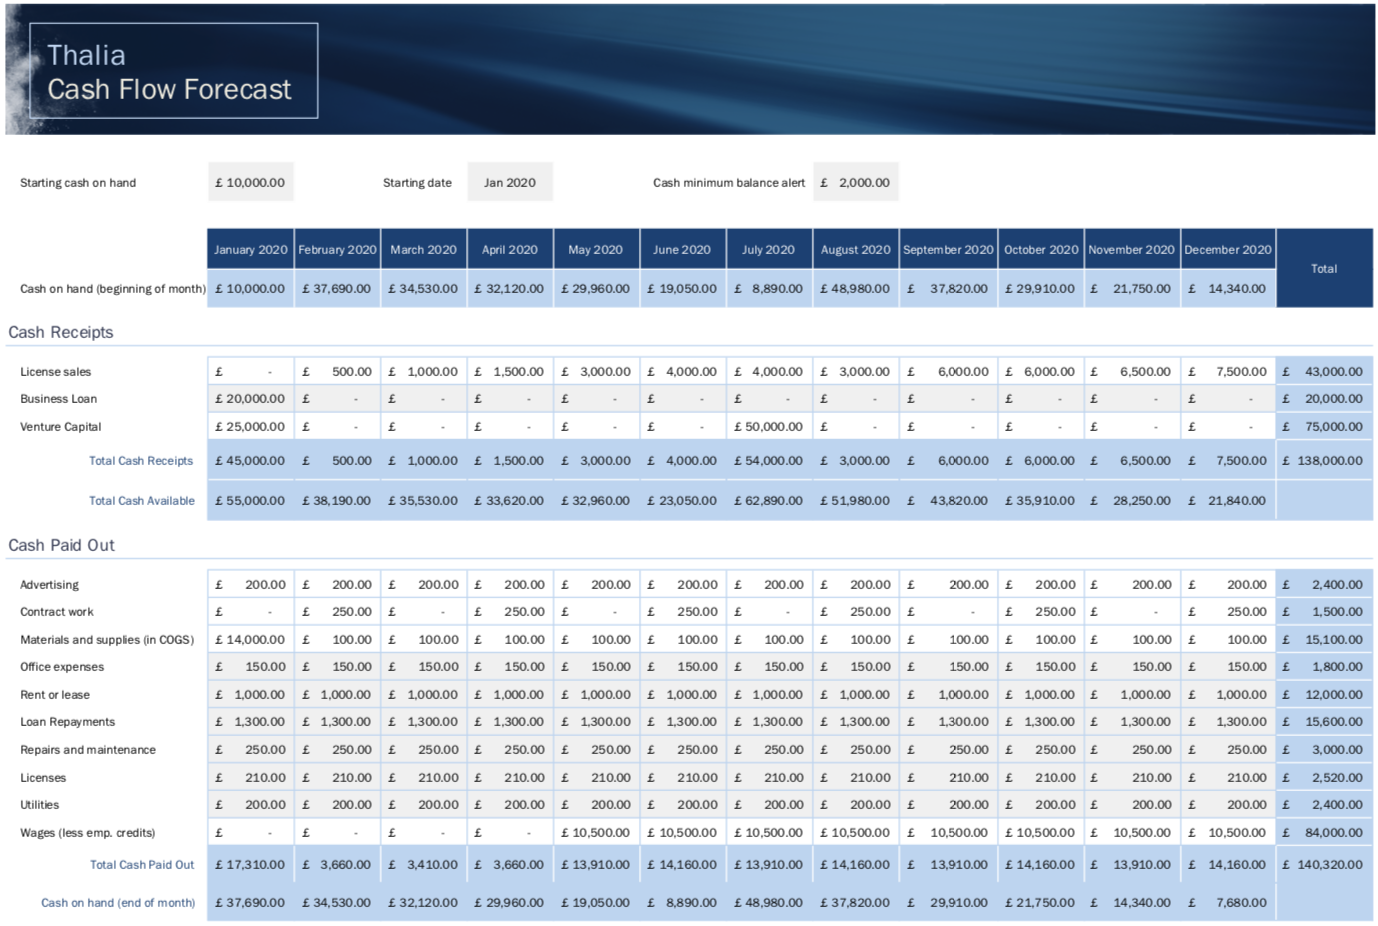
\includegraphics[width=\textwidth]{03Requirements/03Pictures/cash_flow_forecast.png}
\end{figure}

This forecast makes several assumptions that we deem justifiable:

\begin{itemize}
    \item Seed and Series A venture capital investments of a total of £75,000.
    \item Approximately linear growth of license sales throughout the year.
    \item Team members being able to sustain themselves without a salary for the four starting months.
    \item Being able to acquire a £20.000 business loan with less than 5\% interest p.a.
\end{itemize}

These assumptions lead to our company being profitable by mid 2021. Time to profitability of around 18 months is very typical for startups, as shown e.g. by Olsen and Kolvereid \cite{startup_profitability}. While these findings are indicators of economic feasibility, we will have to constantly revise our cash flow forecast to account for changing market conditions and advances in product development.

\subsubsection{Legal}

Fundamentally, backtesting is not considered to encourage purchases or sales of assets. Our company is merely providing information to our customers and thus can not be considered to provide financial advice. Decisions drawn from the information presented by Thalia solely consists of the opinions of our customers and do not reflect the opinions of the Thalia team or any associates. A disclaimer of this form will be placed on our website and within our terms and conditions which have to be accepted by users upon sign up.
Within the framework of the Financial Conduct Authority, our product is understood to provide guidance on investment decisions. Entities offering guidance `are responsible for the accuracy and quality of the information they provide` \cite{fca_guidance_advice}. Thus, it is paramount that the information provided by our tool is accurate.

Our research has not revealed any other potential legal issues with our service. Given correctness of our calculations, we thus consider this project to be legally feasible.

\subsubsection{Operational}

After deployment of our service, we will need to continually update price data for all assets while integrating new assets to stay competitive. For a discussion of how live data is integrated into our service, please refer to the design section concerning the Data Collection module \ref{Data Harvester}. Given that these requirements are the only way in which we deviate from other web applications, we are confident that this project is feasible from an operations standpoint.

\subsubsection{Scheduling}

The Thalia Technical Report established a schedule for this sub-session. The aforementioned strict requirement of correctness of our service makes it difficult to estimate the time required for developing a system component. We are using the Agile development methodology as described in our white paper \cite{WP} as a means of adjusting for this uncertainty. Our previous schedule must then be understood to be less rigid and used instead for orientation of how to prioritise work efforts. Delivery of a correct product is thus ensured at any point. Scheduling issues are therfore less of an issue as reducing the feature specification in favour of accuracy of results is the preferred course of action.

\subsubsection{Conclusion}

The areas in the TELOS analysis yielding questions about the feasibility of this project are Economic and Legal. Accordingly, we have incorporated actions that reduce any potential negative impact of these risks into our strategy. In particular, we will be including legal disclaimers on our website and as part of our terms of service and try to acquire external funding for the initial development stage of our business as soon as possible. We believe that these discussions solidify the case for our project being feasible.

\end{document}
